
%(BEGIN_QUESTION)
% Copyright 2009, Tony R. Kuphaldt, released under the Creative Commons Attribution License (v 1.0)
% This means you may do almost anything with this work of mine, so long as you give me proper credit

Read and outline the ``3-Way Solenoid Valves'' subsection of the ``Solenoid valves'' section of the ``Discrete Control Elements'' chapter in your {\it Lessons In Industrial Instrumentation} textbook.  Note the page numbers where important illustrations, photographs, equations, tables, and other relevant details are found.  Prepare to thoughtfully discuss with your instructor and classmates the concepts and examples explored in this reading.

\underbar{file i04194}
%(END_QUESTION)




%(BEGIN_ANSWER)


%(END_ANSWER)





%(BEGIN_NOTES)

3-way valves are like SPDT switches: one common port switching to one of two other ports:

$$\includegraphics[width=15.5cm]{i04194x01.eps}$$

Typical lables for 3-way valve ports:

\begin{itemize}
\item{} {\bf P} = Pressure (supply)
\item{} {\bf E} or {\bf T} = Exhaust (vent) or Tank
\item{} {\bf C} or {\bf A} = Cylinder or Actuator
\end{itemize}

\begin{itemize}
\item{} {\bf 1} = Common
\item{} {\bf 2} = Port which is open (flowing) when actuated
\item{} {\bf 3} = Port which is open (flowing) when at rest
\end{itemize}

P\&ID symbology for solenoid valves not as descriptive.  Letters such as ``D'' and ``E'' must be drawn next to the valve symbol to denote directions of flow when de-energized and energized, respectively:

$$\includegraphics[width=15.5cm]{i04194x02.eps}$$

\vskip 10pt

Solenoid valve ratings (both fluid and electrical) are important, and typically stamped on a nameplate on the valve.








\vskip 20pt \vbox{\hrule \hbox{\strut \vrule{} {\bf Suggestions for Socratic discussion} \vrule} \hrule}

\begin{itemize}
\item{} {\bf Present a 3-way solenoid valve to students for their inspection, challenging them to identify all ports on the valve.  If practical, set up a power supply to energize the solenoid so they may test its operation by blowing air through the ports in different energization states.}
\item{} What would be a typical application for a three-way solenoid valve?
\item{} Suppose a 3-way valve had no labels on its ports.  Describe a procedure by which you could determine the identities of ports 1 (common), 2 (flowing when actuated), and 3 (flowing at rest).
\item{} Explain why it would be a good idea to connect a {\it commutating diode} across the coil of the ASCO brand solenoid valve shown in the book.
\end{itemize}

%INDEX% Reading assignment: Lessons In Industrial Instrumentation, Solenoid Valves (3-way solenoid valves and symbols)

%(END_NOTES)


